\documentclass[11pt,letterpaper]{article}

\usepackage{graphicx}
\usepackage[margin=1in]{geometry}
\usepackage{amsmath}
\usepackage[T1]{fontenc}
\usepackage[utf8]{inputenc}
\usepackage{authblk}
\usepackage{fancyhdr}  
\usepackage{lastpage}
\usepackage[parfill]{parskip}
\usepackage{subcaption}

\pagestyle{fancyplain}

% Headers
\lhead{}
\chead{}
\rhead{}

% Footers
\lfoot{}
\cfoot{}
\rfoot{\footnotesize Page \thepage\ of \pageref{LastPage}}

\renewcommand{\headrulewidth}{0.0pt} % No header rule
\renewcommand{\footrulewidth}{0.4pt} % Thin footer rule

\title{Analyzing Response to Vehicular Incidents with Tableau}

\author[ ]{Benjamin Bengfort}
\author[ ]{Bor-Chun Chen}
\affil[ ]{Department of Computer Science}
\affil[ ]{University of Maryland}
\affil[ ]{\textit{\{bengfort,bcchen\}@cs.umd.edu}}

\date{Monday, March 2, 2015}



\begin{document}

% Project Requirements

% Use an existing software tool, such as Tableau, Spotfire, QlikView, HCE, TimeSearcher, Treemap, EventFlow, or NodeXL to thoroughly explore a data set of your choice. Report what you found in the form of three headlines that highlight key features, insights, and significant findings. Present 3-6 informative interactive displays (be sure to include legends, make labels readable, and write thoughtful captions) and write 500-1000 words explaining what you have found. At least one of your informative displays should demonstrate coordinated windows or a trellised view. Include your names, email addresses, date, and affiliation. Please describe the data sets you use, indicating number of items and attributes, as well as the source and URL. Critique the tools you used, describing positive aspects, problems you encountered, and suggestions for improvements.

% Your proposal should give a title, the names/emails of the two team members, what software you plan to use, and a few sentences describing the data you will use, plus its source. Your Application Report teammate should be different from your team mates for your Semester Project.

% Deadline: Monday, March 2, 2015 at 6:00pm

\maketitle

\section*{Introduction}

In the State of Maryland, the State Highway Administration (MDSHA) oversees critical responses to events and incidents that occur on the roadways, 24 hours a day - 7 days a week. Maryland has some of the highest density traffic in the United States \cite{terrigno2014traffic}, and includes two major beltways (ring roads) around Baltimore and Washington, I-695 and I-495 respectively. It is therefore critical that first responders are prepared for changing road conditions and are able to plan well in advance for management of routine and extraordinary events. 

At the  University of Maryland, the Center for Advanced Transportation Technology (CATT) Laboratory explores user and visualization driven techniques to solve complex challenges of transportation, safety, and security for the Maryland region. Recently, data collection efforts have improved and large scale probe networks have equipped traffic operations specialists with real time probe data for dynamic monitoring \cite{lund2010dynamic}. The CATT Lab has shown that with effective, real-time visualization of traffic patterns and event analysis, traffic administrators are able to respond more quickly and prepare in advance \cite{pack2010visualization}.

With the support of Maryland State Highway Administration's Incident Management System, the CATT Laboratory has collected 287,712 events that Maryland Coordinated Highway Action Response Teams (CHARTs) responded to from 2011 - 2014. In this paper we use Tableau \cite{mackinlay2007show} to explore patterns in historical responses to these events and critique Tableau's effectiveness as a data analysis tool for response preparedness. We hope to show that a commercial tool for general data analysis like Tableau can provide insights from large amounts of data, and allow first responders to plan and prepare for future events.

\subsection*{Dataset Information}

Our visual exploration utilized a single dataset of events responded to by MDSHA CHARTs across five years, from January 1, 2011 to January 2, 2015\footnote{Special thanks to Michael VanDaniker of the CATT Lab for providing this data}. The events dataset contained 507,685 records, where each record recorded a unique event and response team (e.g. events with multiple responders were shown as two separate records). The dataset used 22 fields to describe the events, however different event types recorded different information, therefore not every record has a complete 22 fields. 

In order to better understand the dataset, we categorized each record attribute as being either an \textit{identifier} or a \textit{descriptor}. Furthermore, we expanded two unique \textit{descriptor} categories for attributes that were not simply text: \textit{time} and \textit{location} attributes. A listing for each field and category is as follows:

\begin{enumerate}
	\item Identifier: \texttt{event\_id}, \texttt{responder\_id}
	\item Time: \texttt{event\_start\_tstamp}, \texttt{closed\_tstamp}, \texttt{notified}, \texttt{responded}, \texttt{departed}, \texttt{removed}
	\item Location: \texttt{location\_name}, \texttt{route\_prefix}, \texttt{route\_name}, \texttt{direction\_description}, \texttt{start\_exit\_name}, \texttt{start\_exit\_number}, \texttt{start\_latitude}, \texttt{start\_longitude}
	\item Description: \texttt{responder\_name}, \texttt{event\_nm}, \texttt{event\_type}, \texttt{incident\_type}, \texttt{op\_center\_description}, \texttt{resource\_type\_description}
\end{enumerate}

All \texttt{event\_id} and \texttt{responder\_id} fields are prefixed with "\texttt{MDOT\_CHART\_}", and further the \texttt{responder\_id} field is post-fixed with an underscore and the \texttt{event\_id}. This led us to believe that  the original data source originally had three normalized tables: \texttt{events}, \texttt{responders}, and a many-to-many join table \texttt{event\_responders}. In total, there are \textbf{287,712 discrete events} in this time period, responded to by \textbf{5,506 responder teams} either singly or in groups.

We also discovered 6 small inner tables - attributes whose unique value count is so small as to be considered types. There are 9 unique \texttt{event\_type} categories: 'Incident', 'Weather service alert', 'Disabled vehicle', 'Action event', 'Special event', 'Planned roadway closure', 'Recurring congestion', 'Safety message', and 'Congestion'. The 'Incident' \texttt{event\_type} is furthermore classed into 18 \texttt{incident\_type} classes that are broadly grouped as 'collision', 'weather', 'policy activity', 'blockage', 'roadwork', and 'other disruption'. Other fields with few unique values included \texttt{op\_center\_description} and \texttt{resource\_type\_description} which appear to describe the responder more than the event. 

In terms of missing values, the field \texttt{removed} was the most unstable, with 98\% of records missing this value. It appears that the \texttt{removed} attribute is associated with a particular \texttt{incident\_type}. Descriptions of location like \texttt{start\_exit\_number} also were null in a significant number of records, probably because these fields require human entry. Because we were especially considering the duration of events, we were pleased to note that the timestamps \texttt{event\_start\_tstamp} and \texttt{closed\_tstamp} appeared in every single record, so we used this field to compute event duration. 

\subsection*{Data Wrangling}

We were particularly interested in using the PostgreSQL data connector that is part of Tableau. The dataset we used was not large, but of a significant enough size that a relational database would make a substantial performance impact. We designed a schema from the CSV data set provided, and wrote a SQL script to import the data using the \texttt{COPY FROM} command. This script can be provided upon request. 

We did note that by loading the data into PostgreSQL, the database did a lot of work for us in terms of data wrangling. For example, the database automatically parsed the date times as they were in a PostgreSQL \texttt{DATETIME WITH TIMESTAMP} format already. When we connected to the database with Tableau, we had no further work in terms of wrangling, which made our lives a lot easier. 


\section*{Insights}

The main focus of our work involved the creation of an interactive tiled overview of the event historical data. Our Tableau dashboard involved three different worksheets, all of which were controlled by two sliders (one for hour of the day, and the other for month of the year), as well as a control to filter by incident type. Figure \ref{fig:dashboard} shows a screenshot of this dashboard at its default setting, all hours of the day, all months of the year, and all event types are selected. By combining a geographic plot of the data with frequency and duration charts, we hoped to show the relationship of seasons and rush hours to incidents, contextualized by areas of high traffic density. 

\begin{figure}
	\centering
    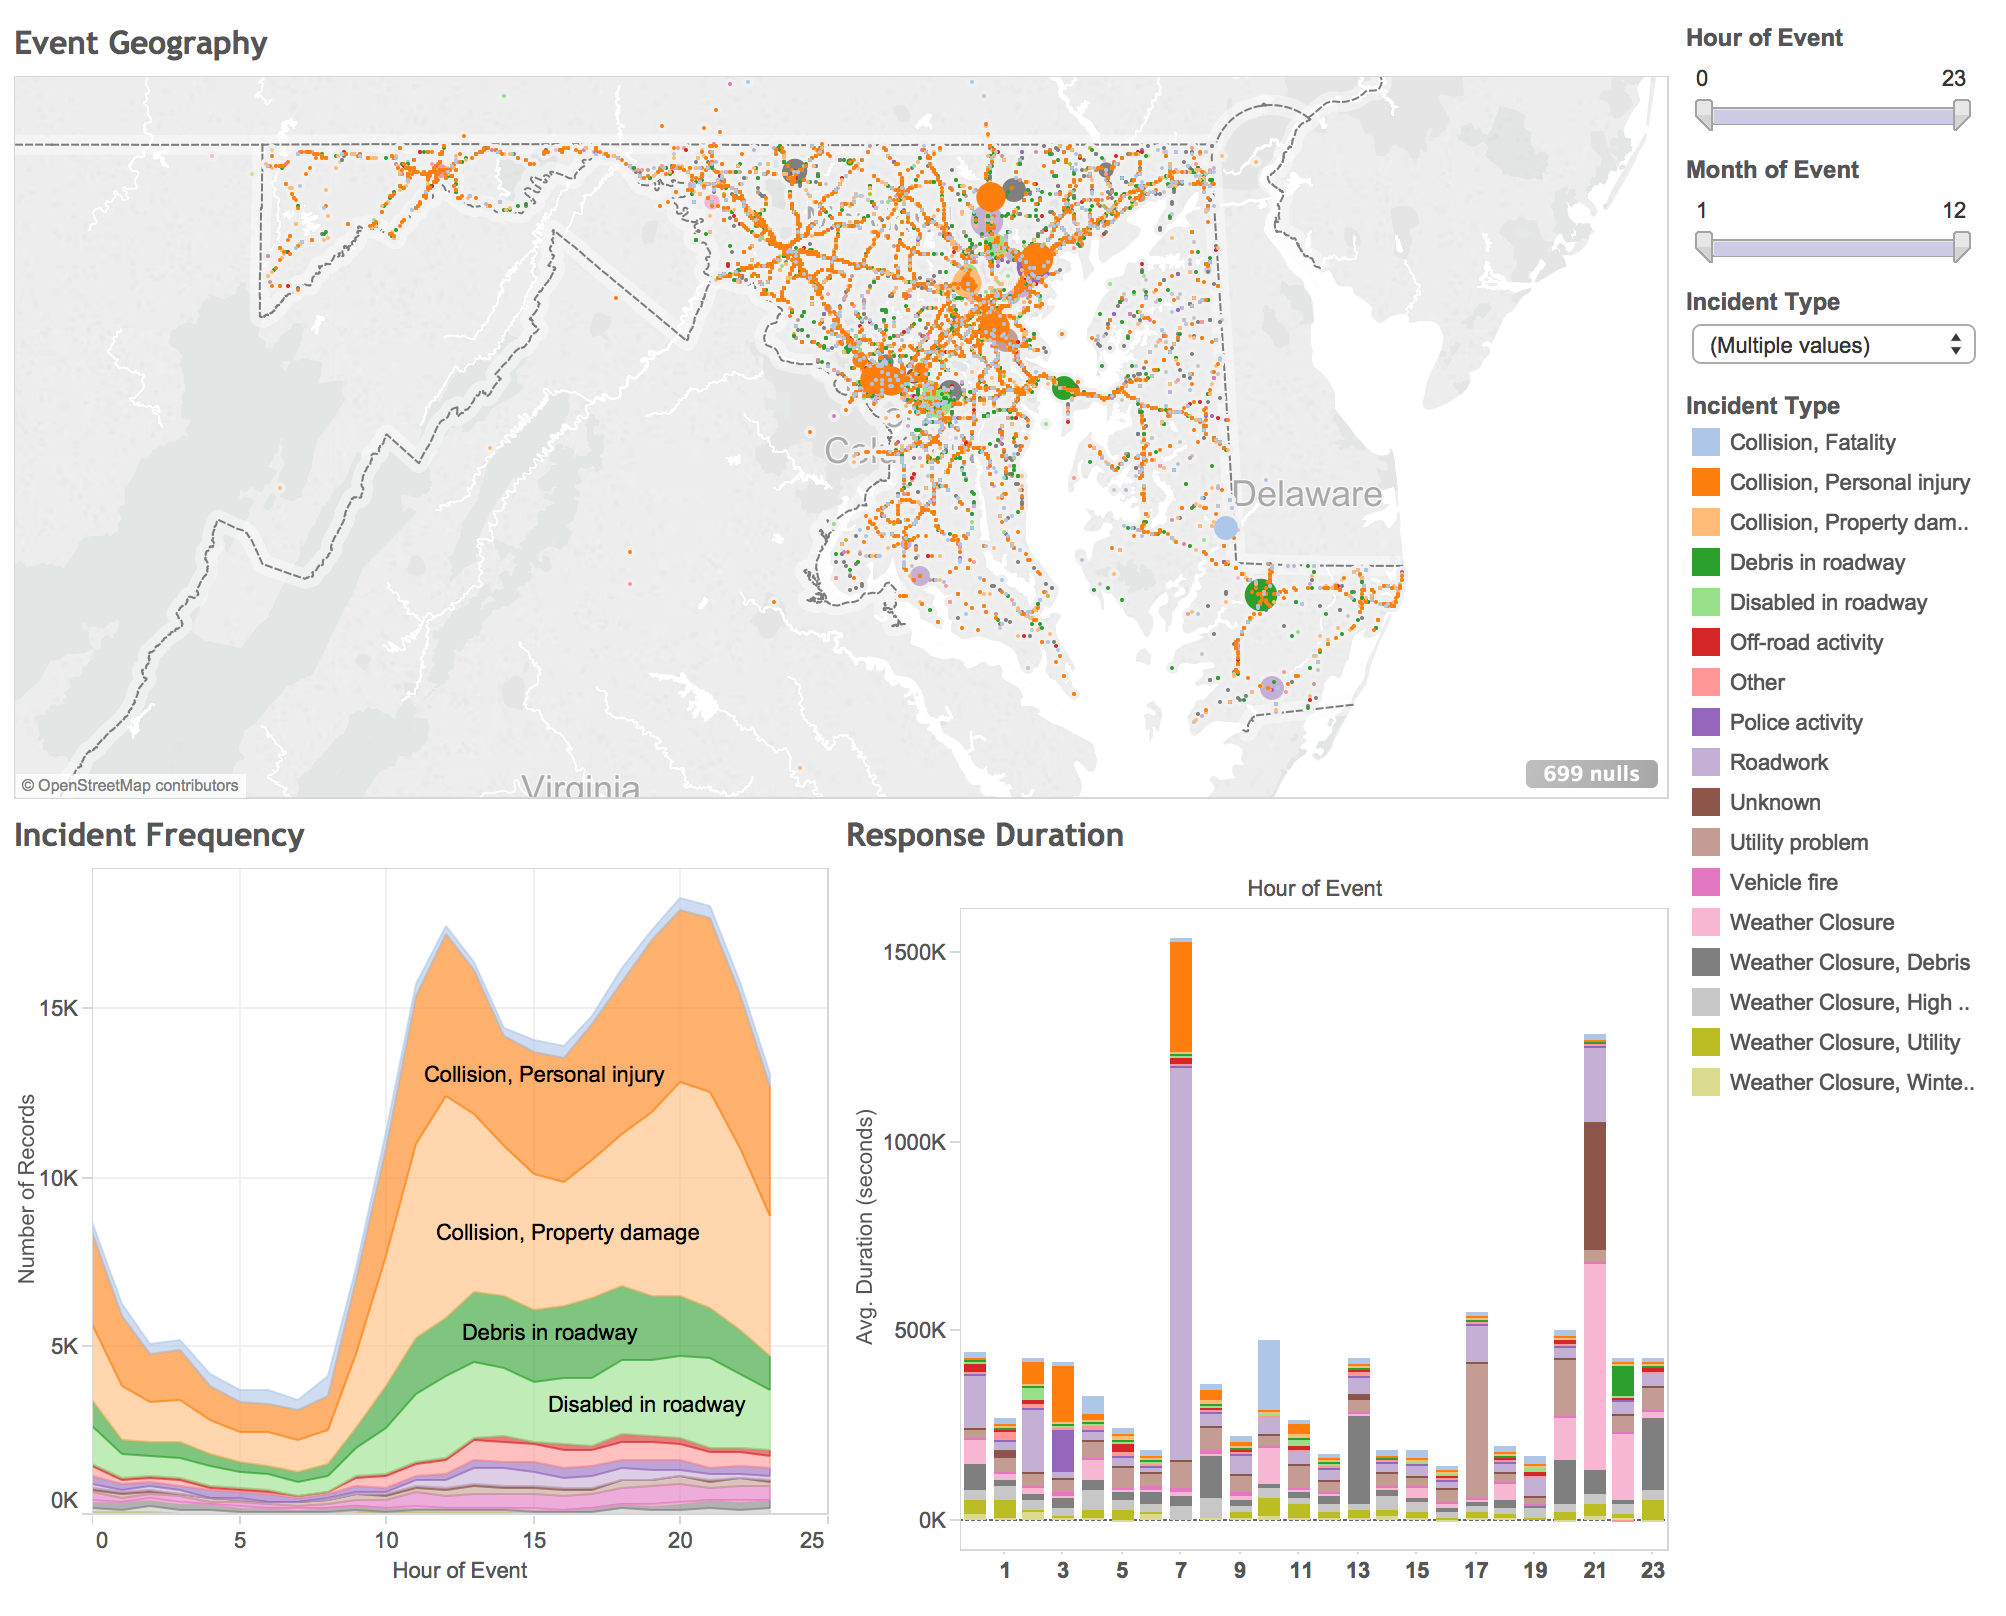
\includegraphics[width=\textwidth]{figures/dashboard.png}
    \caption{\textsf{A tiled, interactive dashboard that is controlled by two sliders and a dropdown filter in order to show the relationship between incident types and the time of day or time of year.}}
    \label{fig:dashboard}
\end{figure}

\subsection*{More CHART Resources are Required near Baltimore in the Evening}

\begin{figure}[h]
	\centering
	\begin{subfigure}{0.49\textwidth}
		\centering
		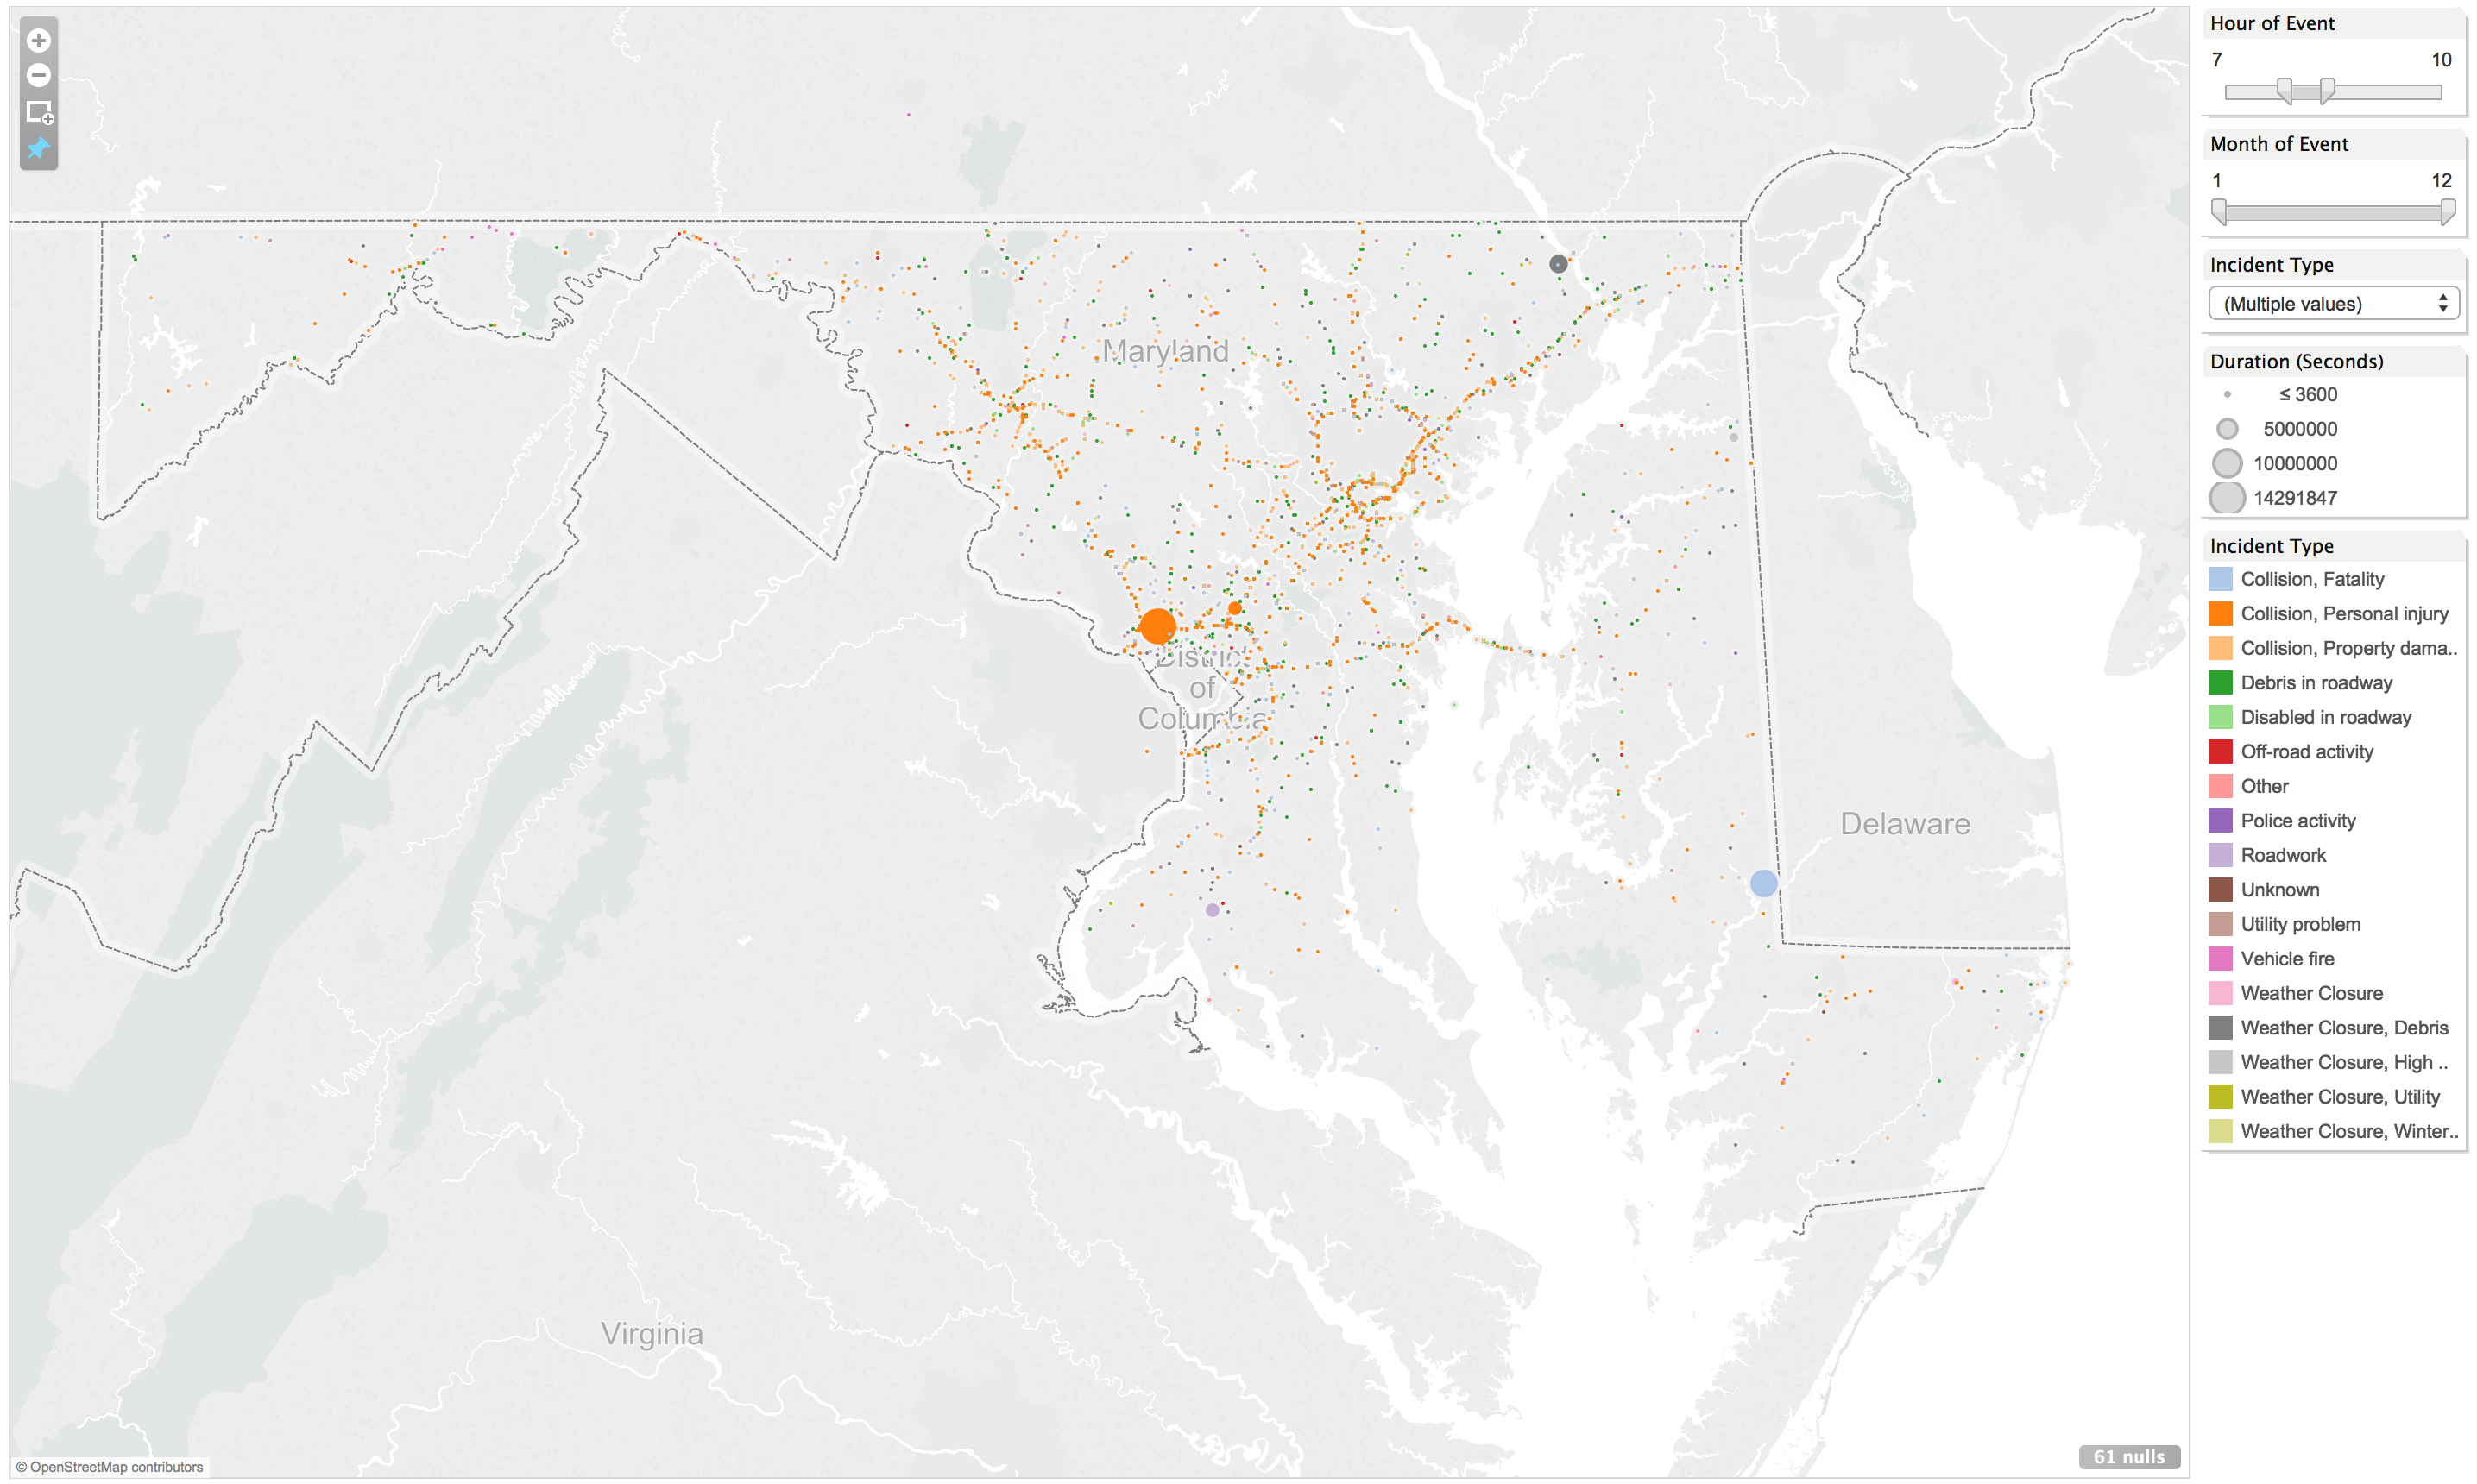
\includegraphics[width=\textwidth]{figures/morning_rush_hour.png}
		\caption{\textsf{Morning Rush Hour}}
        \label{fig:morning_rush_hour}
	\end{subfigure} \hfill
	\begin{subfigure}{0.49\textwidth}
		\centering
		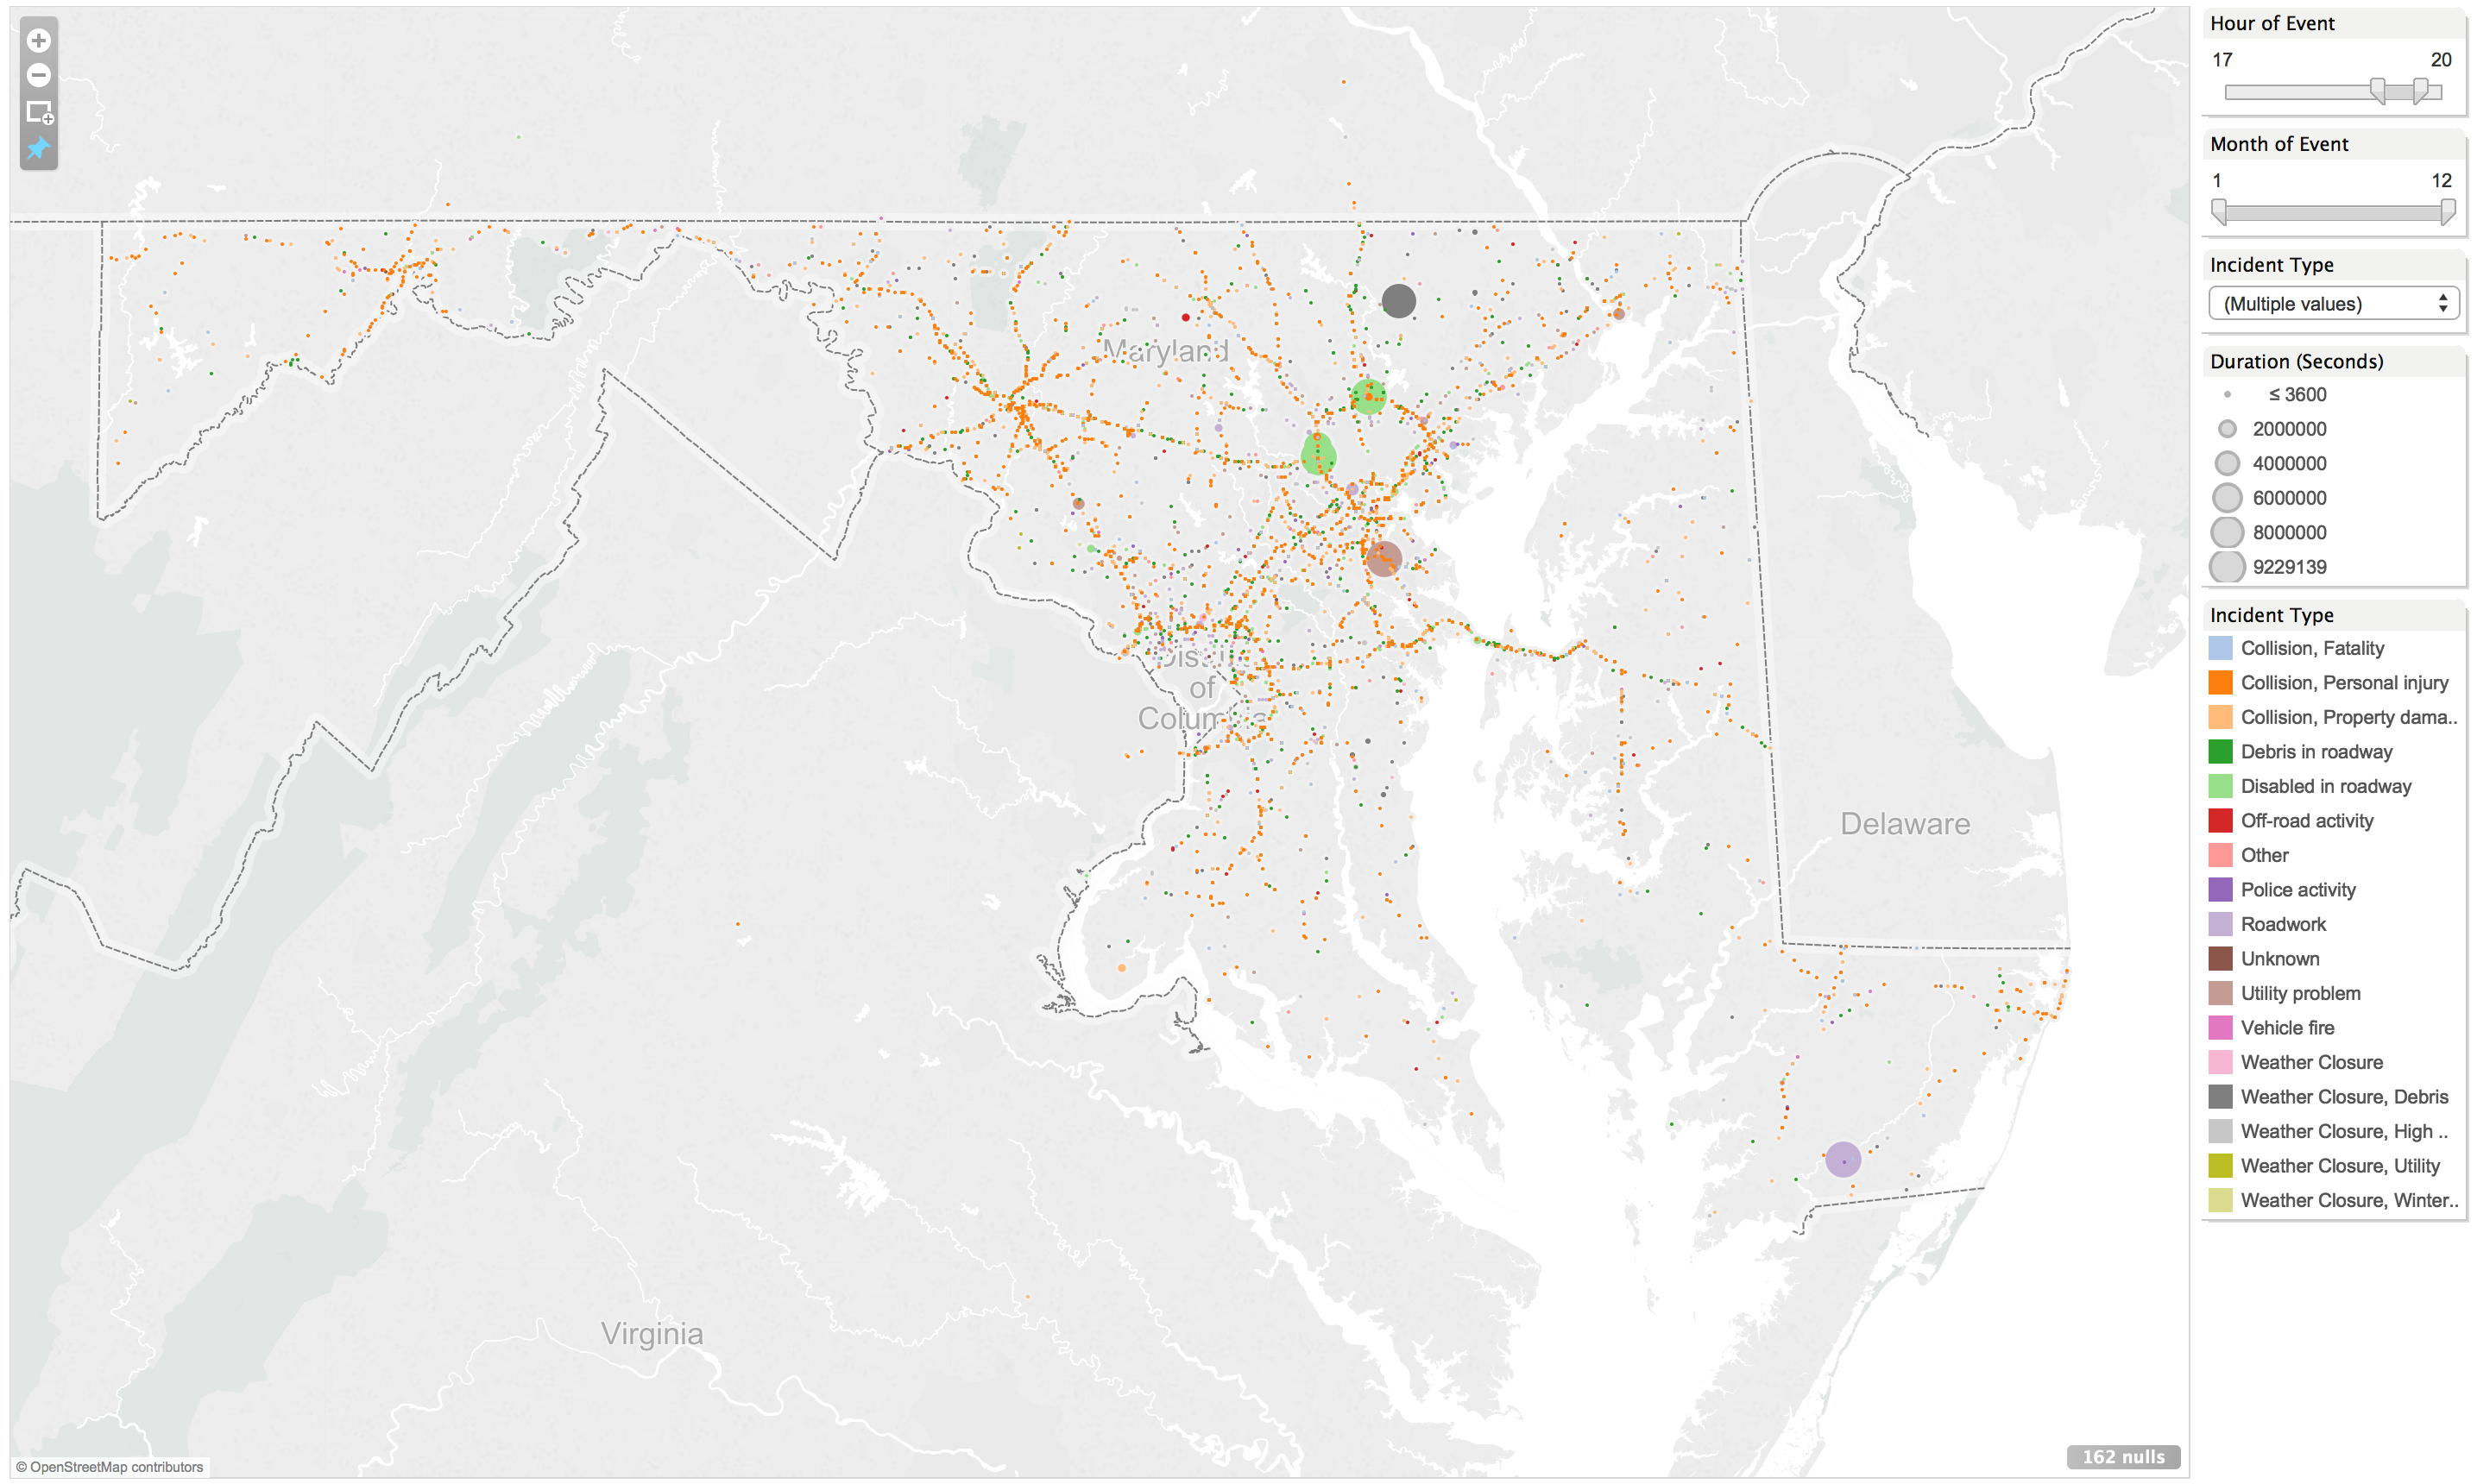
\includegraphics[width=\textwidth]{figures/evening_rush_hour.png}
		\caption{Evening Rush Hour}
        \label{fig:evening_rush_hour}
	\end{subfigure}
    \caption{\textsf{Event location colored by type and sized by duration}}
    \label{fig:geo_rush_hour}
\end{figure}

Understanding non-routine incidents is an important part of planning operations for highway action response teams and scheduling routine action items like roadway closures for repair. In order to better understand the geographic distribution of events and their duration, we plotted each event using their latitude and longitude. Each point was colored by incident type (collisions are orange and weather events are gray) and the size of the point on the map was determined by the relative scale of events. 

Using our time window slider, we inspected the map during the morning rush hour (from 7AM to 10AM) in figure \ref{fig:morning_rush_hour} and again during the evening rush hour (5PM to 8PM) in figure \ref{fig:evening_rush_hour}. Not only is it clear that there are more incidents to respond to in the evening, but those incidents take much longer to respond to and close than incidents in the morning. Geographically speaking, we see heavy incident density along the most traveled roads, but there are far longer incident responses in the north around I-695 and Baltimore than there are in the other parts of the state, including the very high traffic I-495 corridor around Washington, D.C. that includes the I-270 expressway.  

\subsection*{Collisions are Frequent, but Responder Time Dominated by Weather}

\begin{figure}[h]
	\centering
	\begin{subfigure}{0.49\textwidth}
		\centering
		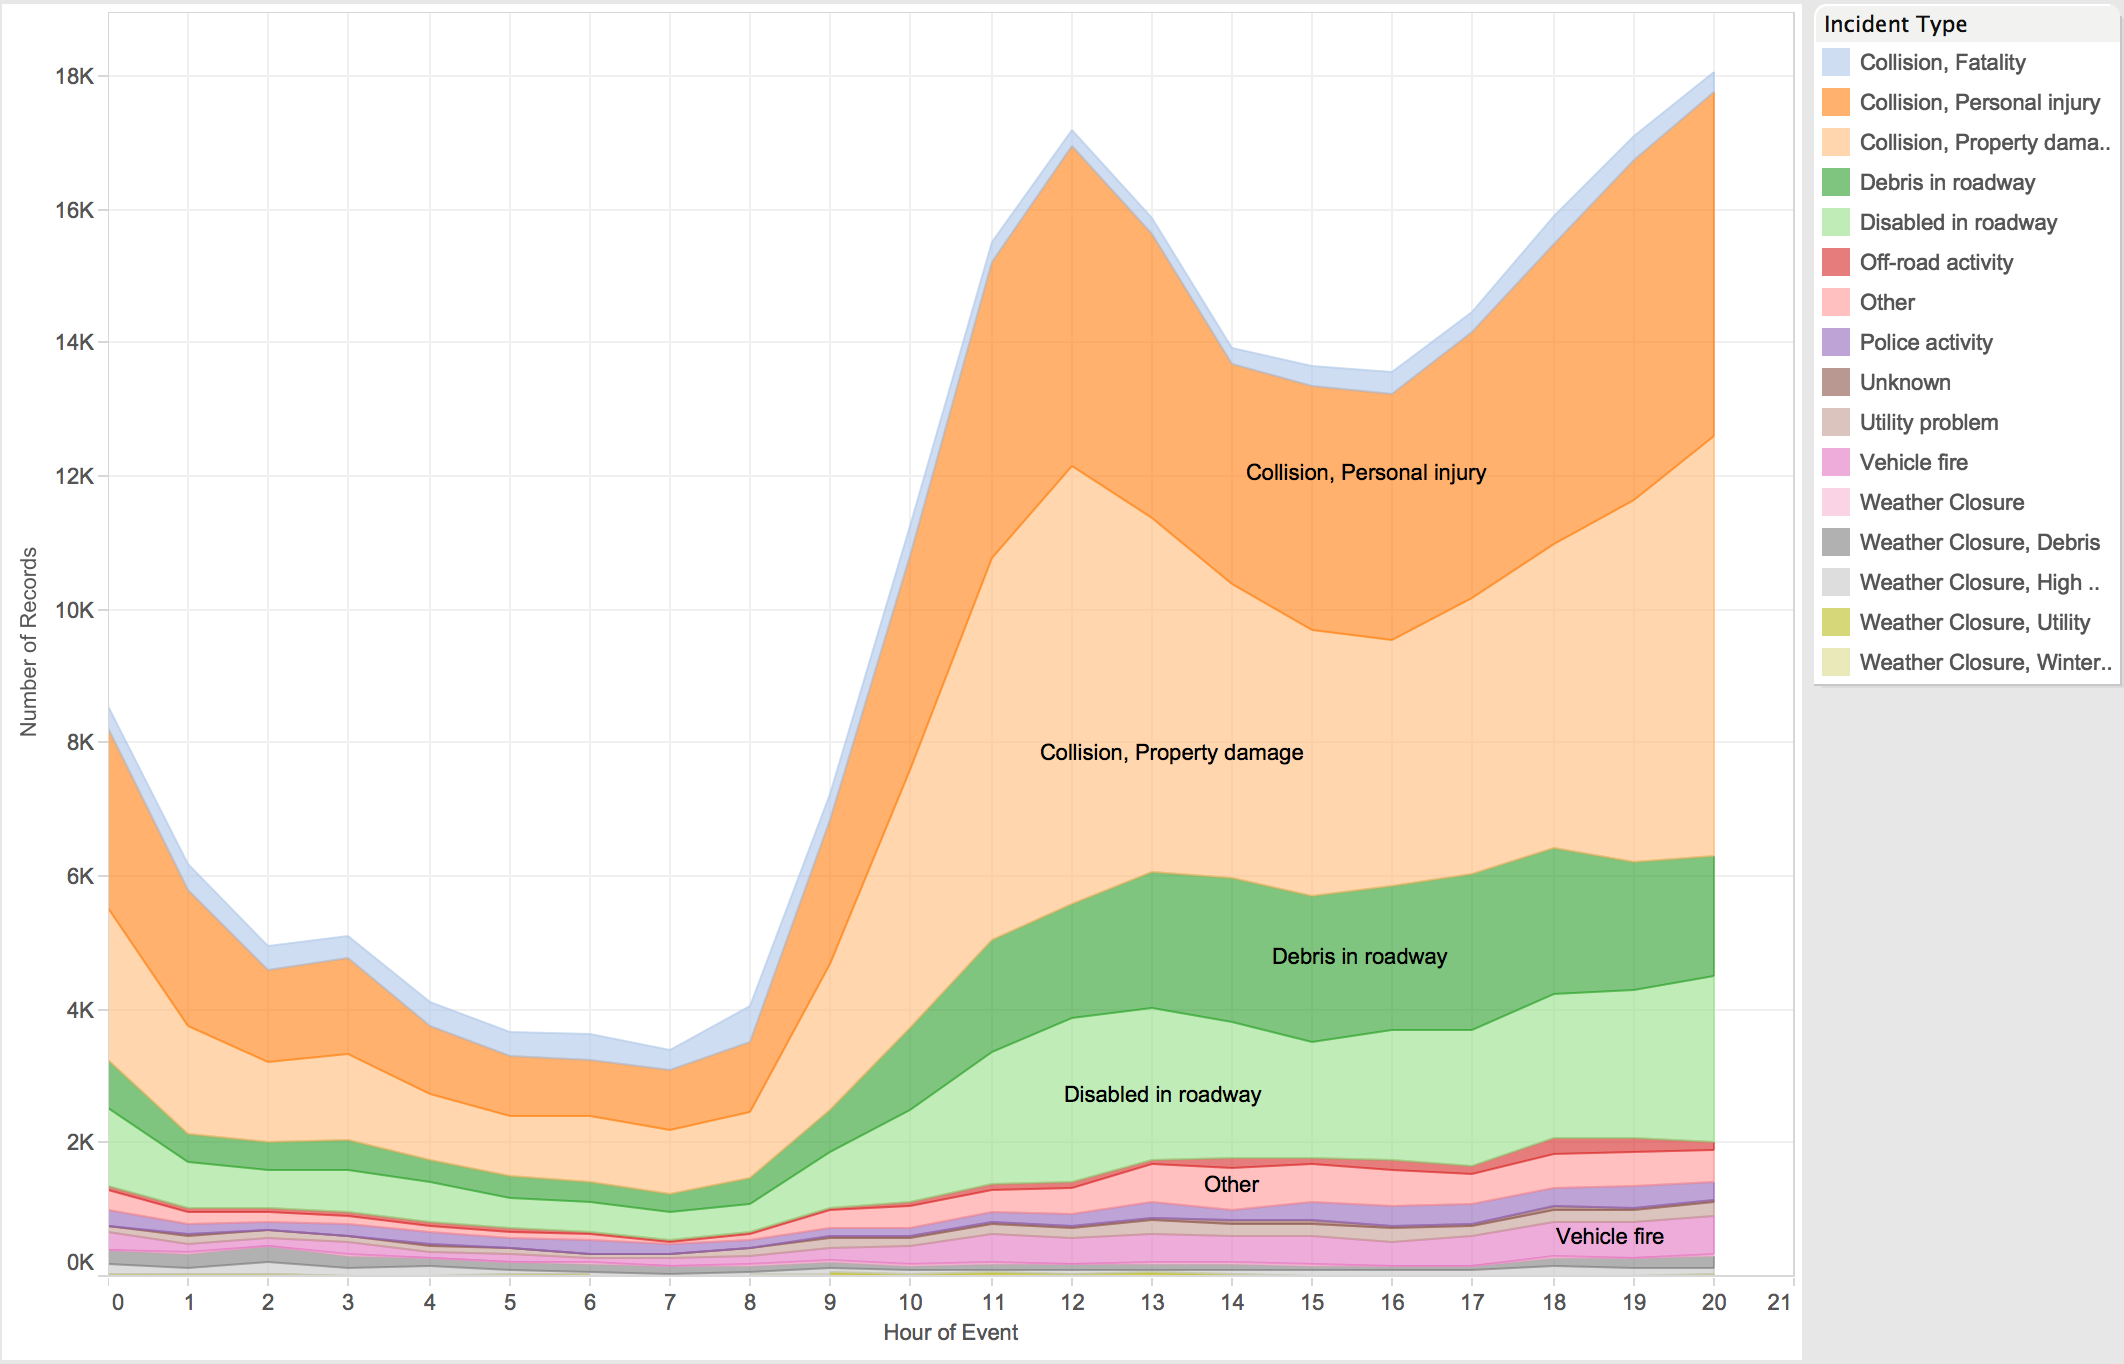
\includegraphics[width=\textwidth]{figures/event_frequency.png}
		\caption{\textsf{Event Frequency}}
        \label{fig:event_frequency}
	\end{subfigure} \hfill
	\begin{subfigure}{0.49\textwidth}
		\centering
		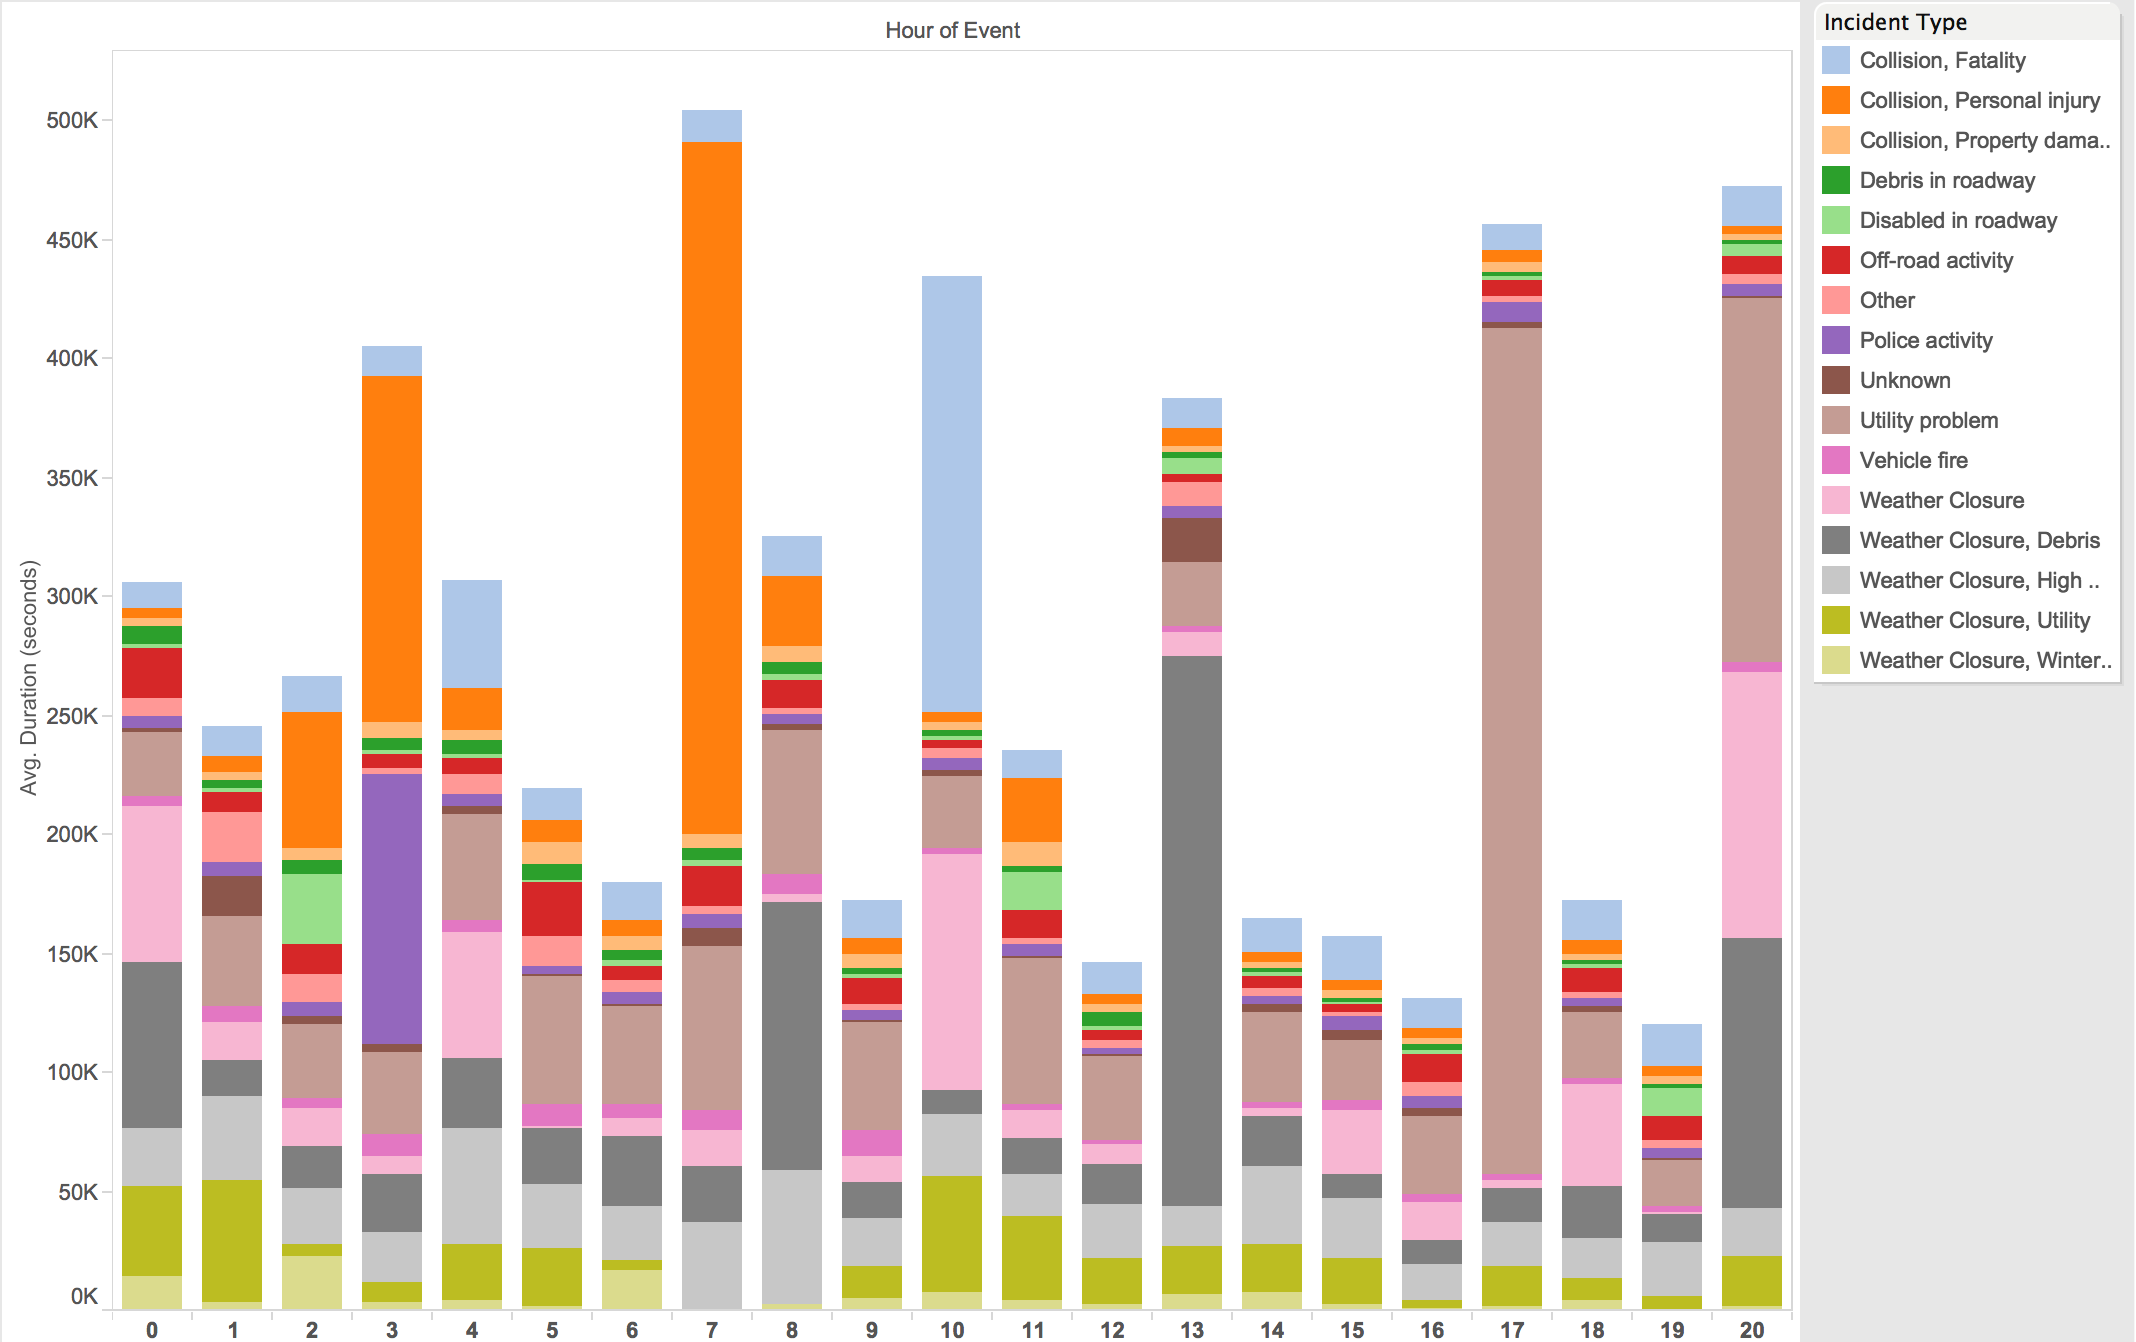
\includegraphics[width=\textwidth]{figures/event_duration.png}
		\caption{Event Duration}
        \label{fig:event_duration}
	\end{subfigure}
    \caption{\textsf{Event frequency and duration by incident type and hour of the day}}
    \label{fig:incident_analysis}
\end{figure}

We continued our theme of scheduling and planning resources based on historical events by comparing the frequency and duration of events by time of day. Our hypothesis was that the time of day was more important to response time and event duration than the incident type itself. E.g. incident types would have a mostly constant response time relative to their frequency. In order to explore this we created two visualizations - the first, figure \ref{fig:event_frequency}, was an area histogram that showed for each hour of the day, how many incidents of each type there were. This graph clearly reinforces our earlier discovery that most incidents happen in the afternoon or evening. It also became clear that the types of responses in the afternoon or evening dealt with collisions, particularly ones where someone might be injured (and to a lesser extent, to clear debris from the road). 

Our second chart, figure \ref{fig:event_duration}, told a slightly different story. In this chart we plotted a combined bar chart of the average response duration per hour of the day, by incident type. In this chart, we see that average collision response time is the highest in the morning, and that total average response time (across all incident types) is very similar between the morning and evening rush hours. In fact, responses to events caused by utilities or weather dominated the average response time overall, not responses to the most frequent types of events! Moreover, average response time to collisions and debris (the most frequent types of events) is overall very small relative to other events. 

Our chart was also quick filtered by seasonality - that is we displayed data for a sliding window of months as well as hours. We revised our hypothesis when we saw that weather related events are most common during the winter, and that their average duration is highest afternoon. We suspect this is because if there is winter related weather in the morning, school and work are usually delayed or canceled, whereas weather in the afternoon or evening causes more significant delays to responses. 

\subsection*{Summer Weather Events Have Highest Impact}

The Maryland/DC area is not especially known for having severe winters, but is known for having severe summer weather as tropical storms and hurricanes move along the East Coast from the warmer waters of the Caribbean. We hypothesized that because of this, summer weather would have the most impact. To analyze the patterns of seasonality to incident type, we plot the cumulative total of each event type with respect to month of the year as shown in figure \ref{fig:weather}. Indeed, we find that during the months of June, July, August, and September high water and debris events are the most frequent and have the most impact on the response time of first responders. 

\begin{figure}[h]
	\centering
	\begin{subfigure}{0.49\textwidth}
		\centering
		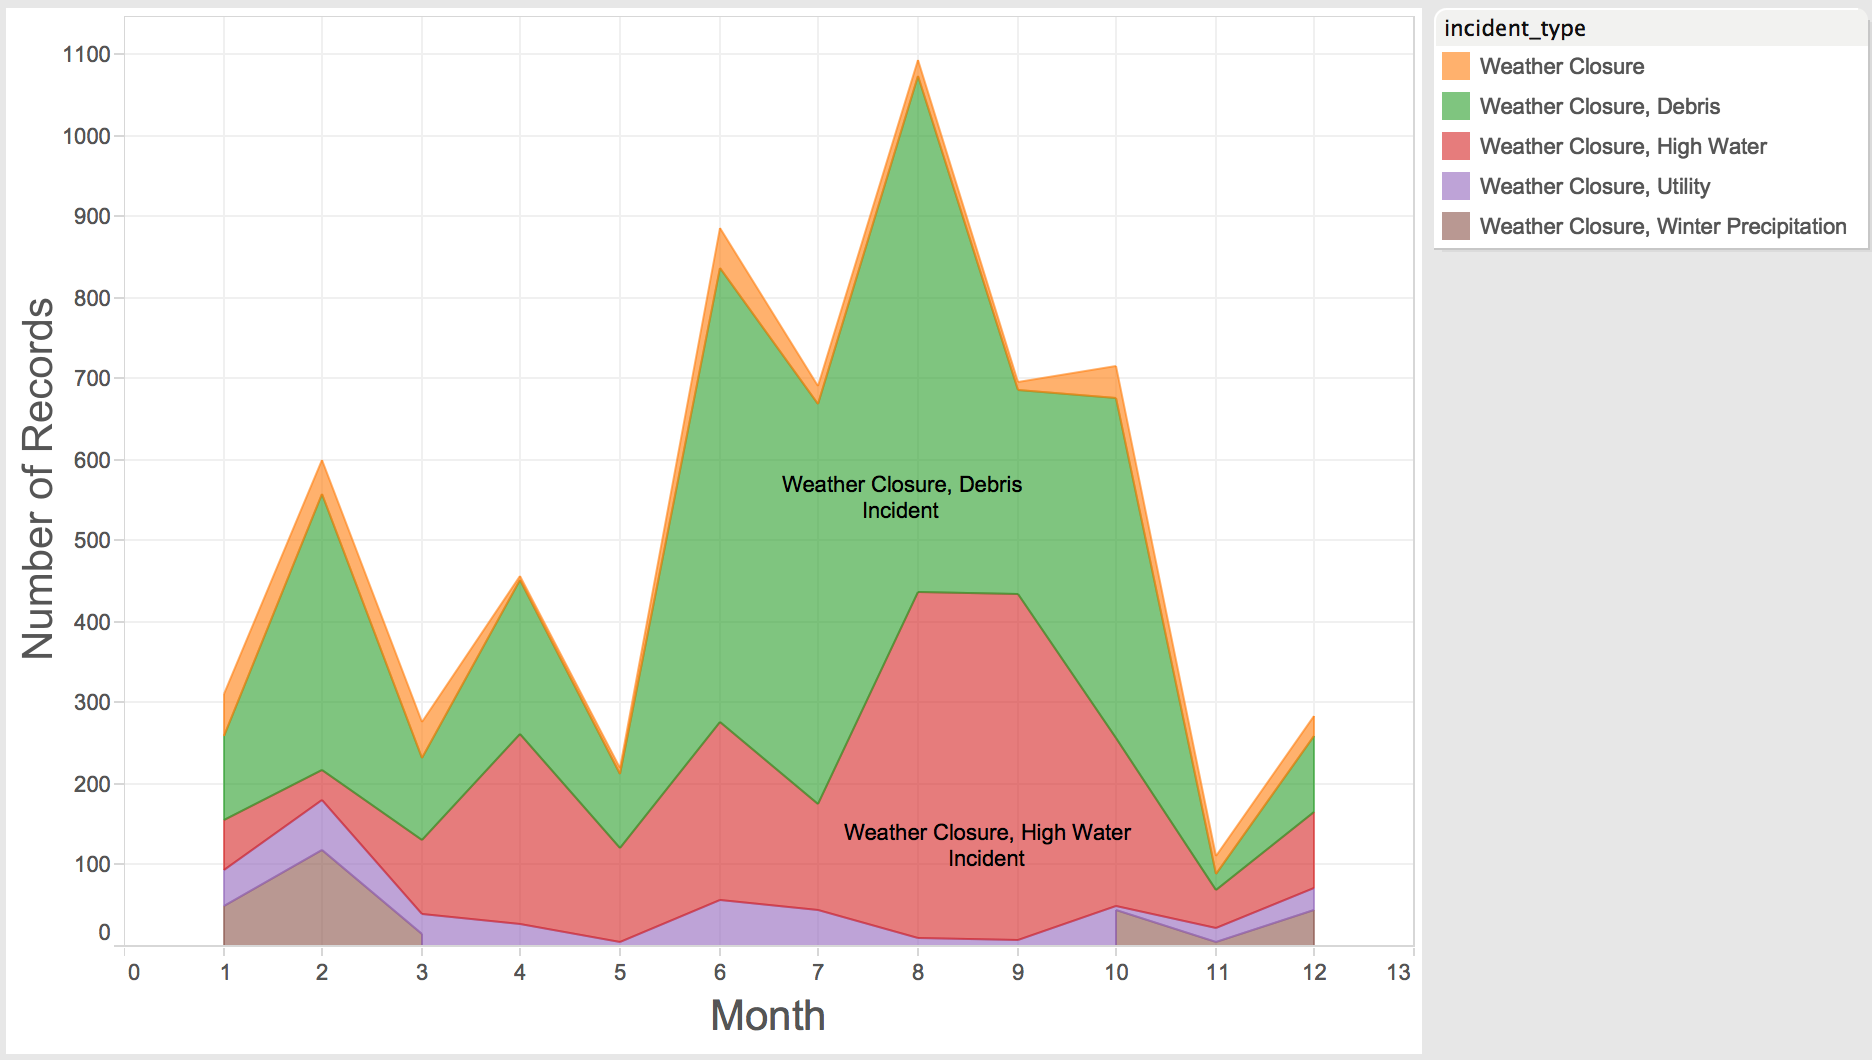
\includegraphics[width=\textwidth]{figures/weather.png}
    	\caption{\textsf{Incident Type}}
	    \label{fig:weather}
	\end{subfigure} \hfill
	\begin{subfigure}{0.49\textwidth}
		\centering
		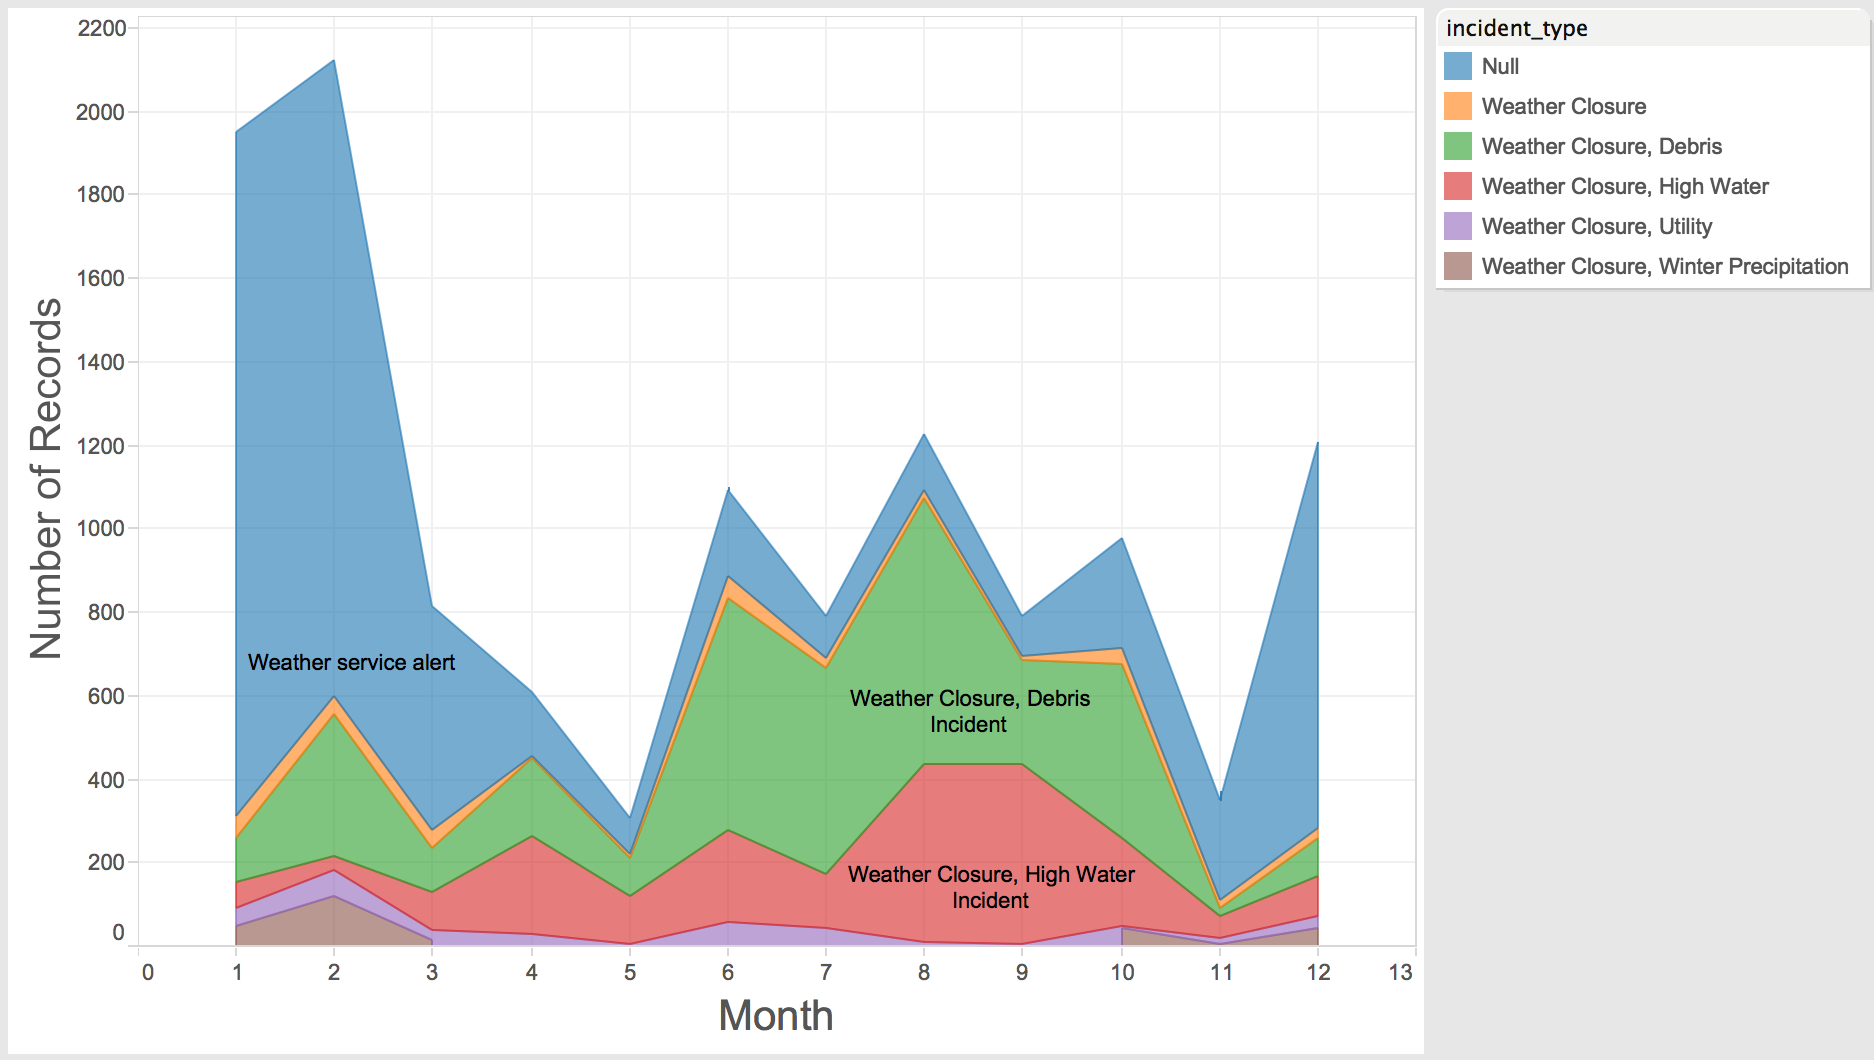
\includegraphics[width=\textwidth]{figures/weather_event.png}
		\caption{Event Type}
        \label{fig:weather_event}
	\end{subfigure}
    \caption{\textsf{The effect of seasonality on incident and event types}}
    \label{fig:weather_types}
\end{figure}

Even so, "weather service alerts" are more frequent during the winter months of December, January, and February as shown in figure \ref{fig:weather_event}. Winter weather events have an effect on response in terms of average event duration. By playing with the interactive dashboard, we found that winter weather has the highest impact in the afternoon, rather than in the morning, although there are peaks during both the morning and evening rush hours. In this case, it is not a matter of frequency of event, but rather severity. These seems to be inline with weather patterns in the Maryland/DC area and CHART response teams have also clearly kept this in mind for scheduling in the past. According to our historical data, routine incidents (road work, debris clearing, etc.) tend to happen more frequently during the summer. 

\subsection*{Fatality Rate Changes with the Seasons}

We wrapped up our exploration of the time of day and time of season compared to event frequency with a novel visualization as shown in Figure \ref{fig:circles}. These graphs plot the time of day along the X-axis, and the month of the year on the Y-axis. Every point on the graph is colored by incident type and sized by frequency. We found that when we included all incident types on this graph we had a colorful, if not informative view of the data that we had already shown - namely that the time of day has a bigger impact on the frequency of events than the season. 

However, when we began to filter the graph to look at specific event types, interesting correlations began to emerge. For example, if you show only the roadwork even type, you can see that most roadwork is conducted during the summer. Even more interestingly, if you compare roadwork, police action, and fatal collisions you begin to see a pattern emerge as shown in figure \ref{fig:circles_death}. Fatalities (the blue circles) are most common in the winter (October through February) and in the early morning hours and seem to correlate when there is both police action and road work, but not when there is only one or the other. 

In figure \ref{fig:circles_seasons}, we can see another visualization that shows our earlier hypothesis - that most weather related incidents happen in the morning or at night during the summer. And that winter weather, if it happens, occurs in the afternoon usually during February. The graphs we have displayed are a bit too small to see this in great detail, but we gained these insights by playing with the controls of Tableau. As static representations we'll admit that these charts are difficult to read. However, when you can see changes occur as you add or remove filters, it is much easier to come up with novel insights! 

\begin{figure}[h]
	\centering
	\begin{subfigure}{0.49\textwidth}
		\centering
		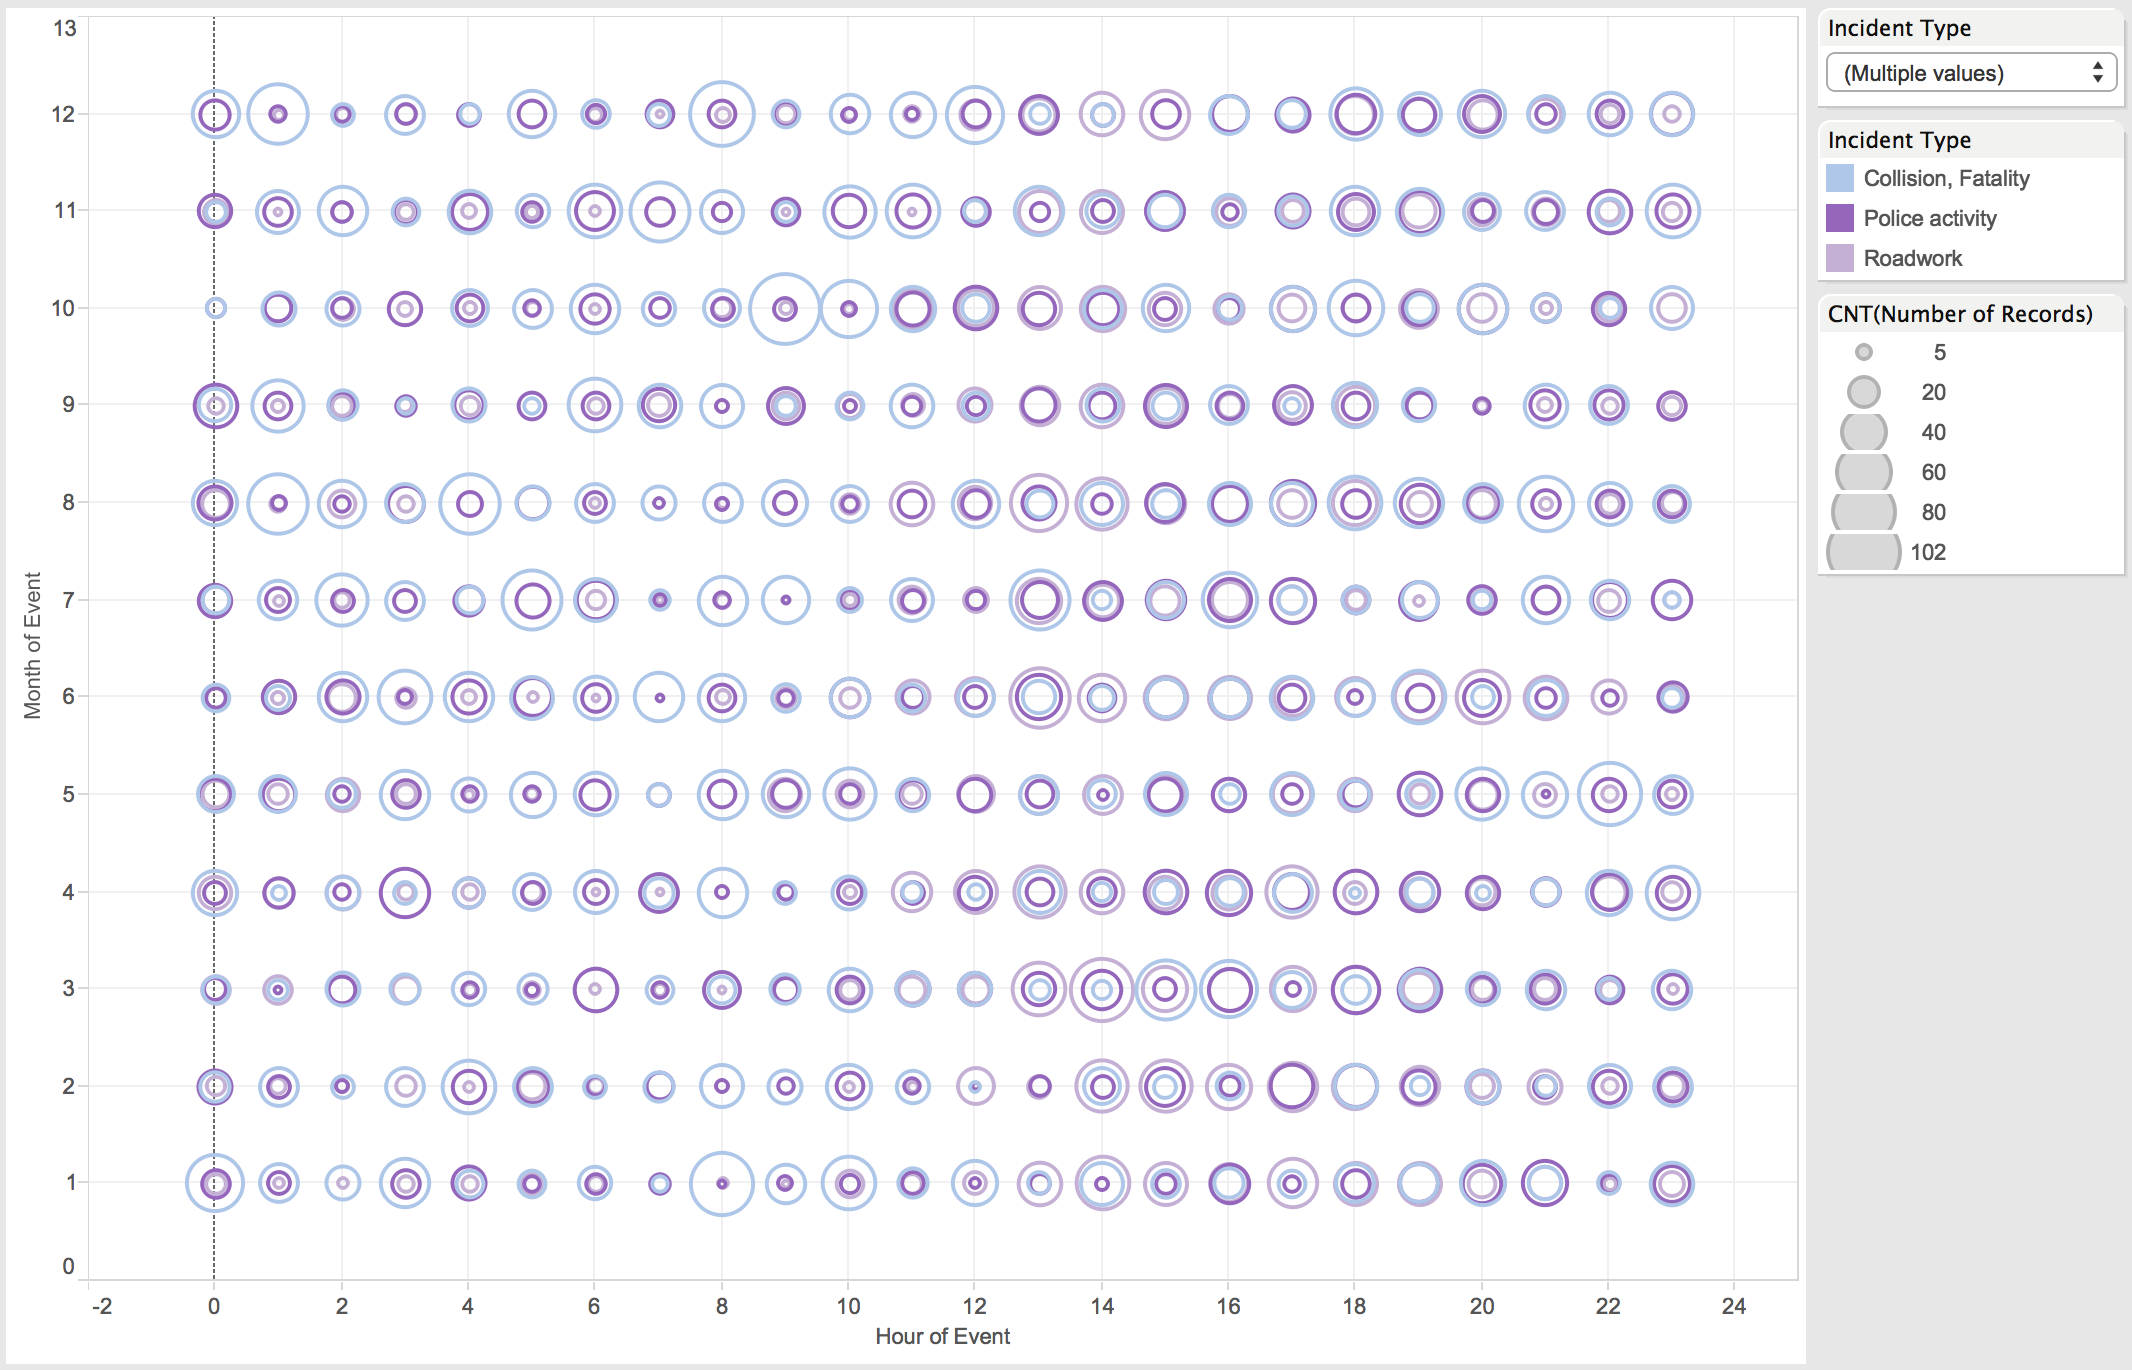
\includegraphics[width=\textwidth]{figures/circles_death.png}
    	\caption{\textsf{Fatalities, Police Action, and Roadwork}}
	    \label{fig:circles_death}
	\end{subfigure} \hfill
	\begin{subfigure}{0.49\textwidth}
		\centering
		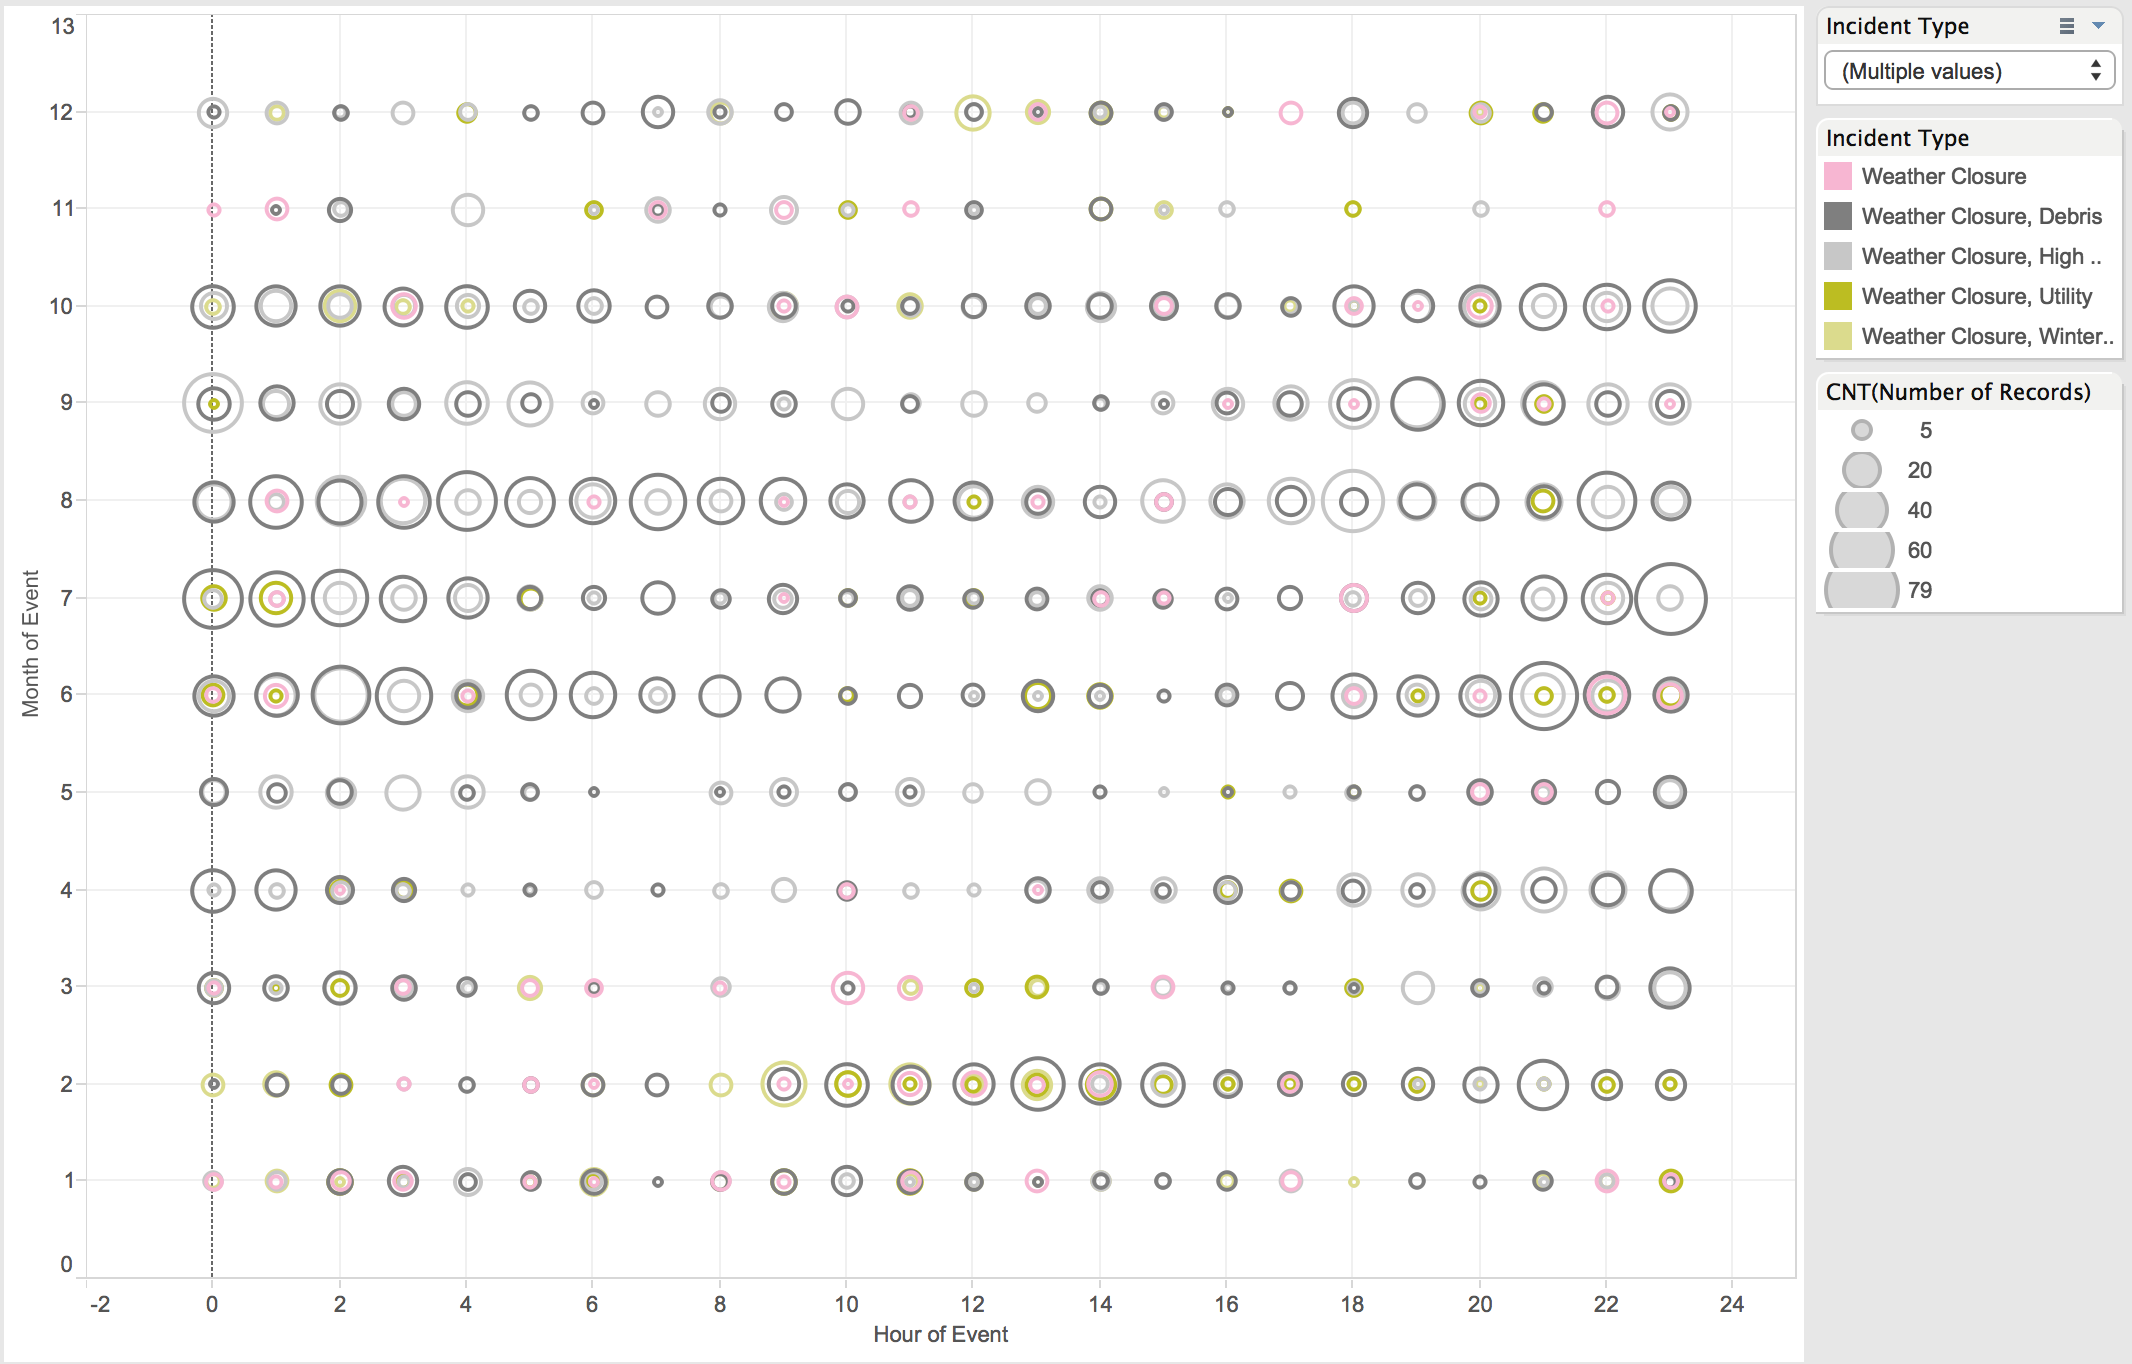
\includegraphics[width=\textwidth]{figures/circles_seasons.png}
		\caption{Weather Incidents}
        \label{fig:circles_seasons}
	\end{subfigure}
    \caption{\textsf{Hour of the Day by Season for Fatalities and Weather Incidents}}
    \label{fig:circles}
\end{figure}



\subsection*{CHART Unit 9741 has the Quickest Transit Time}


For our last exploration, we changed tack a bit. We wanted to determine which CHART had the best transit time on average where transit time is the difference between the time they were notified and when they arrived on the scene. Transit times could be affected by rush hours, proximity, as well as incident type (e.g. collisions are usually responded to immediately, whereas debris clearing may require special equipment). Transit time may even be affected seasonally. However, we discovered that the two timestamps that transit time depend on, namely \texttt{notified} and \texttt{responded} were really only saved for events involving collisions or extraordinary events, not routine events. Additionally, there was bad or missing data that caused negative or null transit times, and some responders who caused outlier data by only responding to few events.  

Figure \ref{fig:transit_time_responder} shows the top 19 responders that have at least 100 event responses and an average transit time of faster than five minutes. Here we see that CART Unit 9741 has an average transit response time of 97.3 seconds! Second place is slightly over 2 minutes- CHART Unit 9500, and finally the quickest responders can be on scene around 4 minutes. These response times have a lot to do with units being on the road when calls come in, and with incident types that do not require advanced preparation. 

Figure \ref{fig:transit_time_event} shows the average response time by incident type. Planned roadway closure have the fastest response times, but this might be bad data, as again, responders have advanced knowledge of these types of incidents. Events that are unplanned take on average 750 seconds to respond to, where disabled vehicles have the fastest response time, and "special events" have the longest. Interestingly congestion also have a long response time, probably caused by the incident itself!

\begin{figure}[h]
	\centering
	\begin{subfigure}{0.49\textwidth}
		\centering
		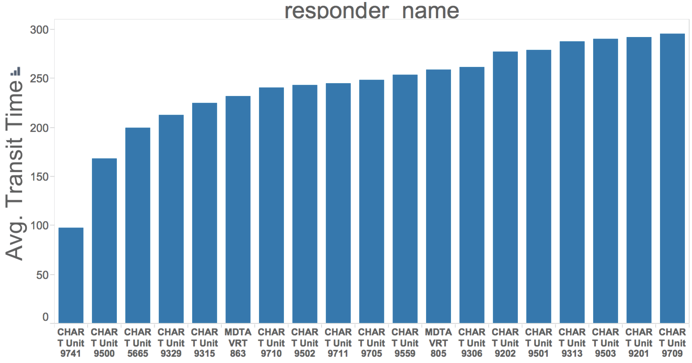
\includegraphics[width=\textwidth]{figures/transit_time_responder.png}
		\caption{\textsf{Average Transit Time per Responder}}
        \label{fig:transit_time_responder}
	\end{subfigure} \hfill
	\begin{subfigure}{0.49\textwidth}
		\centering
		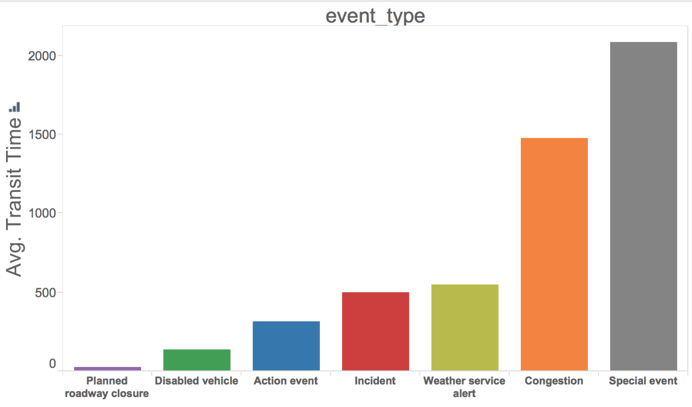
\includegraphics[width=\textwidth]{figures/transit_time_event.png}
		\caption{Average Transit Time by Incident Type}
        \label{fig:transit_time_event}
	\end{subfigure}
    \caption{\textsf{Average Transit Time for Responders and by Events}}
    \label{fig:transit_time}
\end{figure}

\section*{Critique}

Our primary use of Tableau focused on using the tool for larger data analyses and visualizations that cannot be accomplished with traditional tools like Microsoft Excel. In particular, we wanted to compare Tableau to using a powerful relational database and simply making queries upon it. In general we liked the visual aspects of data exploration in Tableau. A common workflow for our team in the past was to export the results of aggregation style SQL queries from the database into a tool like matplotlib or ggplot to get a visual sense of what was happening. Tableau allowed us to quickly see and react to our data in a meaningful way. 

What was most compelling about Tableau was the ease with which we were able to connect to the database. Although this is not an out-of-the-box feature, a simple download from the Tableau website gave us the functionality we needed. Loading the data was a cinch. We were quickly able to get histograms and other data analyses running. 

More complex tasks like putting together a dashboard, filtering globally, and changing the dimensions of the data had a steeper learning curve. However, compared to other tools like Excel or even SQL by itself - it was not a burden. The drag-and-drop interface became particularly intuitive once we realized we could click and edit the details after quickly getting close to where we needed to be by simply dragging. 

However, more complex computations turned out to be more difficult in Tableau. A major part of our analysis involved computing durations from two timestamps. Unfortunately we could find no way to do this with the functions available to us in Tableau - not even a calculated field would make the computation. Luckily, Tableau supports making raw SQL queries directly against the database, so we were able to make our computations using the more powerful data backend. Folks using CSV or other data sources would have been out of luck however! 

The fact that Tableau allowed us to connect to more powerful analytical tools solved many of our challenges, but we also noticed that as time went on our queries got slower and slower. I had to restart Tableau several times when a query wouldn't finish. Executing the same query on the database directly only took a few seconds. Tableau is probably caching the connection or doing some other memory unfriendly things that probably have to be resolved. Tableau is also famous for being able to connect to so called "Big Data" applications like Spark, but clearly Tableau works best on small to medium size data sets, not larger ones like the kind relational databases store. 

\section*{Conclusion}

In this paper we used Tableau to create an interactive visualization that mapped historical trends of responses by CHART teams to events on Maryland highways. Our interactive dashboard contained three panes, a geographical event pane, an incident by frequency pane, and an incident by duration pane. Using two sliding controls for time of day and time of year, as well as a drop down filter for event type, we were able to explore trends on different event types in the context of high volume times (rush hours) and seasonality (winter vs. summer). 

\bibliography{paper}
\bibliographystyle{plain}

\end{document}